% !TEX root = ./document.tex

\documentclass{article}
\usepackage{mystyle}
\usepackage{myvars}


%-----------------------------

\begin{document}

	\maketitle
	\thispagestyle{firststyle}


%-----------------------------
%	ABSTRACT
%-----------------------------

	\begin{abstract}
		\noindent [TODO ]
	\end{abstract}

%-----------------------------
%	TEXT
%-----------------------------


	\section{Introduction}
	\label{sec:intro}

			\paragraph{}
			[TODO ]


	\section{Supervised Learning}
	\label{sec:supervised-learning}

		\paragraph{}
		[TODO ]


		\paragraph{Overfitting}
		\label{paragraph:overfitting}
		[TODO ]

		\paragraph{Error Measures}
		\label{paragraph:error-measures}
		[TODO ]

		\begin{itemize}
			\item
				\textbf{Error Rate}:
				[TODO ]

			\item
				\textbf{Resubstitution error}:
				[TODO ]

			\item
				\textbf{Generalization Error}:
				[TODO ]

		\end{itemize}

		\paragraph{Experimental Strategies}
		\label{paragraph:experimental-strategies}
  	[TODO ]

		\begin{itemize}
			\item
				\textbf{Holdout}:
				[TODO ]

			\item
				\textbf{Repeated Holdout}:
				[TODO ]

			\item
				\textbf{Cross Validation}:
				[TODO ]

			\item
				\textbf{Repeated Cross Validation}:
				[TODO ]

		\end{itemize}

		\subsection{Decision Trees}
		\label{sec:decision-trees}

			\paragraph{}
			Decision trees are classifiers that works splitting the instances between the branches of a tree according to its attributes and assigning the feature's attribute in the leafs of the tree. An scheme of this structure is been included in the figure \ref{fig:decision-tree-concept}. Decision trees can represent logic functions. It tend to ovefit the data so the advanced heuristics try to avoid this problem.

			\begin{figure}
				\centering
				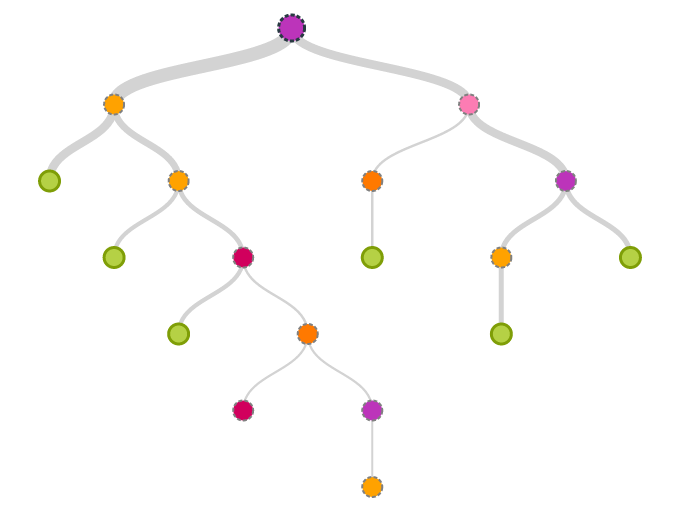
\includegraphics[width=.4\textwidth]{decision-tree-concept}
				\caption{General concept of Decision Tree. Figure from \cite{bigml:a-new-way-to-visualize-decision-trees}}
				\label{fig:decision-tree-concept}
			\end{figure}


			\subsubsection{Information Theory}
			\label{sec:information-theory}

				\paragraph{}
				Most popular decision trees use information theory heuristics. It's heuristics is based on the information generated by an attribute respect to the feature's attribute. In the equation \eqref{eq:gain-heuristic} $D$ is refered to the feaure's attribute and $A$ to the current attribute to be examined. Note that the cardinalities ($card()$) and proportions ($p()$) is been updated according to dataset instances to be examined.

				\begin{align}
				\label{eq:information-heuristic}
					I(D) &= - \sum_{i \in card(D)}  p(d_i) * log_2(p(d_i)) \\
				\label{eq:rest-heuristic}
					Rest(A) &= \sum_{j \in card(D|A)} \frac{card(D|A_j)}{card(D)} * I(D|A_j) \\
				\label{eq:gain-heuristic}
					Gain(D, A) &= I(D) - Rest(A)
				\end{align}

				\paragraph{}
				There is another heuristic who also uses the cardinality to give advantage to attributes with few categories. This heuristic callec \emph{Information Gain Ratio} is shown at the ecuation \eqref{eq:gain-ratio-heuristic}.

				\begin{align}
				\label{eq:gain-divisor-heuristic}
					GainDivisor(D,A) &= - \sum_{j \in card(D|A)}\frac{card(D|A_j)}{card(D)} * log_2\bigg(\frac{card(D|A_j)}{card(D)}\bigg)\\
				\label{eq:gain-ratio-heuristic}
					GainRatio(D,A) &= \frac{Gain(D,A)}{GainDivisor(D,A)}
				\end{align}

				\paragraph{}
				The technique implemented by \emph{C4.5} to deal with numeric attributes is the binary discretization by intervals distributing the values in two categories. The partition is selected picking the point where the attribute $Gain()$ is maximized. One of the points where the feature changes it value.

			\subsubsection{ID3}
			\label{sec:id3-tree}

				\paragraph{}
				ID3 algorithm builds a tree selecting the attribute who maximizes $Gain()$ function respecto de the feature's attribute. It only works with nominal data and removes the attributes that have already been used. When there is no more attributes to select, it label the branch with the feature of the remainder instances.

				\paragraph{}
				The algorithm uses the bias concept refered as the a-priori intuitions used to learn concepts. The \textbf{inductive bias} used by \emph{ID3} is divided in two parts: the \emph{representational bias} who is related with de hypotesis space (logic functions), and the \emph{preference bias} who is based in the idea that the important caracteristics will be placed at the top of the tree (because of the $Gain()$ heuristic and the Breadth-first search) that has as consequence the tendency of generate low level trees.

			\subsubsection{C4.5}
			\label{sec:c45-trees}

				\paragraph{}
				C4.5 is an extension of ID3 tree. It includes some improvements like branch pruning, working with numerical attributes and unknown values. The pruning works in post-pruning mode, i.e. the tree is generated and after is pruned. The heuristic use to determine if branch is pruned is the improve of pesimistic error rate. There are two pruning operations:

				\begin{itemize}
					\item \textbf{Subtree Replacement}: Consist of remove the selected subtree and assign the most frecuent feature to this leaf.
					\item \textbf{Subtree raising}: Consis on replace a tree by one of it's childrens and redistribute the instances. The operation is expensive.
				\end{itemize}

				\paragraph{}
				Unknown values are trated spliting the selection between branches and assigning probabilities to each of them. The feature where the instance is classified is the one who maximized the probability. During the train period attributes with unknown values are penalized.

		\subsection{Rule Based Systems}
		\label{sec:decision-trees}

			\paragraph{}
			[TODO ]

			\subsubsection{1R}
			\label{sec:1r-rule-based}

				\paragraph{}
				[TODO ]

			\subsubsection{PRISM}
			\label{sec:prism-rule-based}

				\paragraph{}
				[TODO ]

			\subsubsection{IREP}
			\label{sec:irep-rule-based}

				\paragraph{}
				[TODO ]

			\subsubsection{RIPPER}
			\label{sec:ripper-rule-based}

				\paragraph{}
				[TODO ]

			\subsubsection{PART}
			\label{sec:part-rule-based}

				\paragraph{}
				[TODO ]

		\subsection{Instance Based Learning}
		\label{sec:decision-trees}

			\paragraph{}
			[TODO ]

			\subsubsection{K - Nearest Neighbors}
			\label{sec:knn}

				\paragraph{}
				[TODO ]

			\subsubsection{IB3}
			\label{sec:ib3}

				\paragraph{}
				[TODO ]

		\subsection{Bayes Learning}
		\label{sec:decision-trees}

			\paragraph{}
			[TODO ]

			\subsubsection{Naive Bayes}
			\label{sec:naive-bayes}

				\paragraph{}
				[TODO ]

			\subsubsection{K2}
			\label{sec:k2-bayes}

				\paragraph{}
				[TODO ]

			\subsubsection{TAN}
			\label{sec:tan-bayes}

				\paragraph{}
				[TODO ]

		\subsection{Linear Classifiers}
		\label{sec:decision-trees}

			\paragraph{}
			[TODO ]

			\subsubsection{Linear Regression}
			\label{sec:linear-regression}

				\paragraph{}
				[TODO ]

			\subsubsection{Logistic Regression}
			\label{sec:logistic-regression}

				\paragraph{}
				[TODO ]

			\subsubsection{Support Vector Machines}
			\label{sec:svm}

				\paragraph{}
				[TODO ]


		\subsection{Neural Networks}
		\label{sec:neural-networks}

			\subsubsection{Perceptron model}

			\begin{figure}
				\centering
				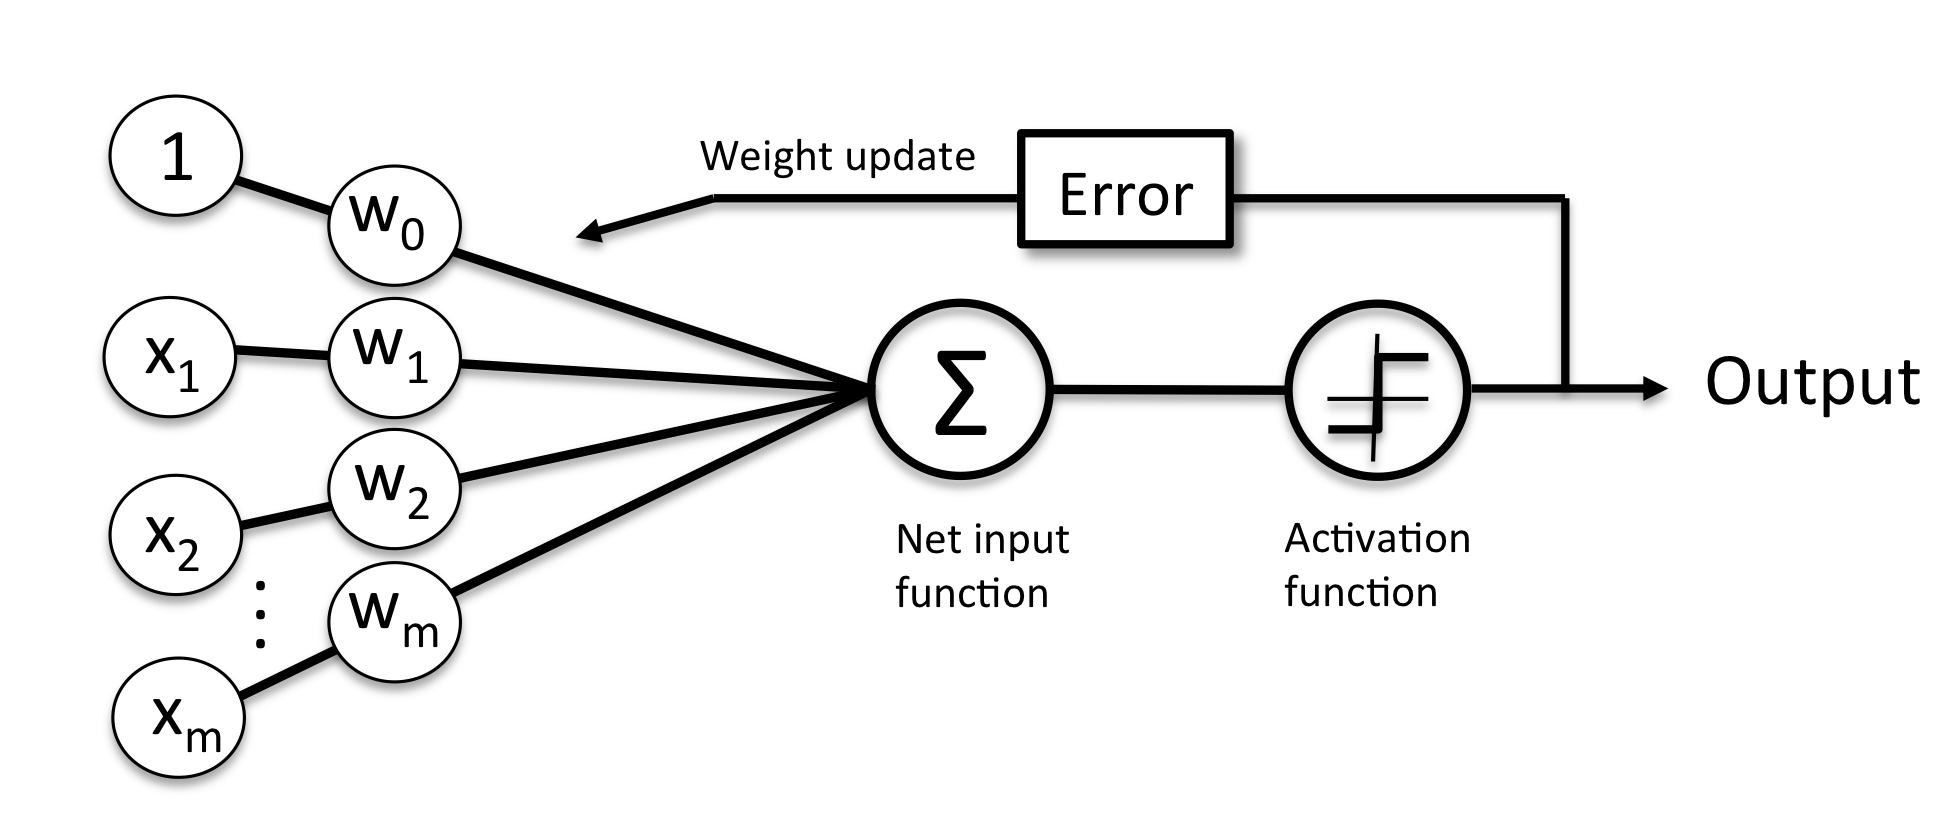
\includegraphics[width=.4\textwidth]{perceptron-concept}
				\caption{General concept of perceptron}
				\label{fig:perceptron-concept}
			\end{figure}

			\paragraph{Perceptron's structures}
			\begin{equation}
				w = \begin{bmatrix}
						w_1 \\
						\vdots \\
						w_m
					\end{bmatrix}, x =
					\begin{bmatrix}
						x_1 \\
						\vdots \\
						x_m
					\end{bmatrix}
			\end{equation}

			\paragraph{Ouput equation}
			\begin{equation}
				z = w_1 x_1 + \dots + w_m x_m = \boldsymbol{w^T x}
			\end{equation}


			\paragraph{Activation function}

			\begin{figure}
				\centering
				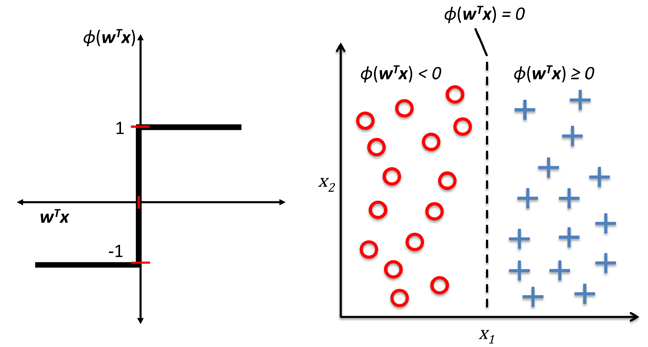
\includegraphics[width=.4\textwidth]{activation-function}
				\caption{Activation function}
				\label{fig:activation-function}
			\end{figure}

			\begin{equation}
				\phi(z) = \begin{cases}
					1 &\mbox{if } z \geq \theta \\
					-1 &\mbox{otherwise}
				\end{cases}
			\end{equation}

			\paragraph{Update of weight vector}

			\begin{align}
					w_j &:= w_j + \Delta w_j \\
					\Delta w_j &= \eta(y^{(i)} - \hat{y}^{(i)}) x^{(i)}_j
			\end{align}

			\subsubsection{Adaptive linear neurons (ADALINE)}

			\begin{figure}
				\centering
				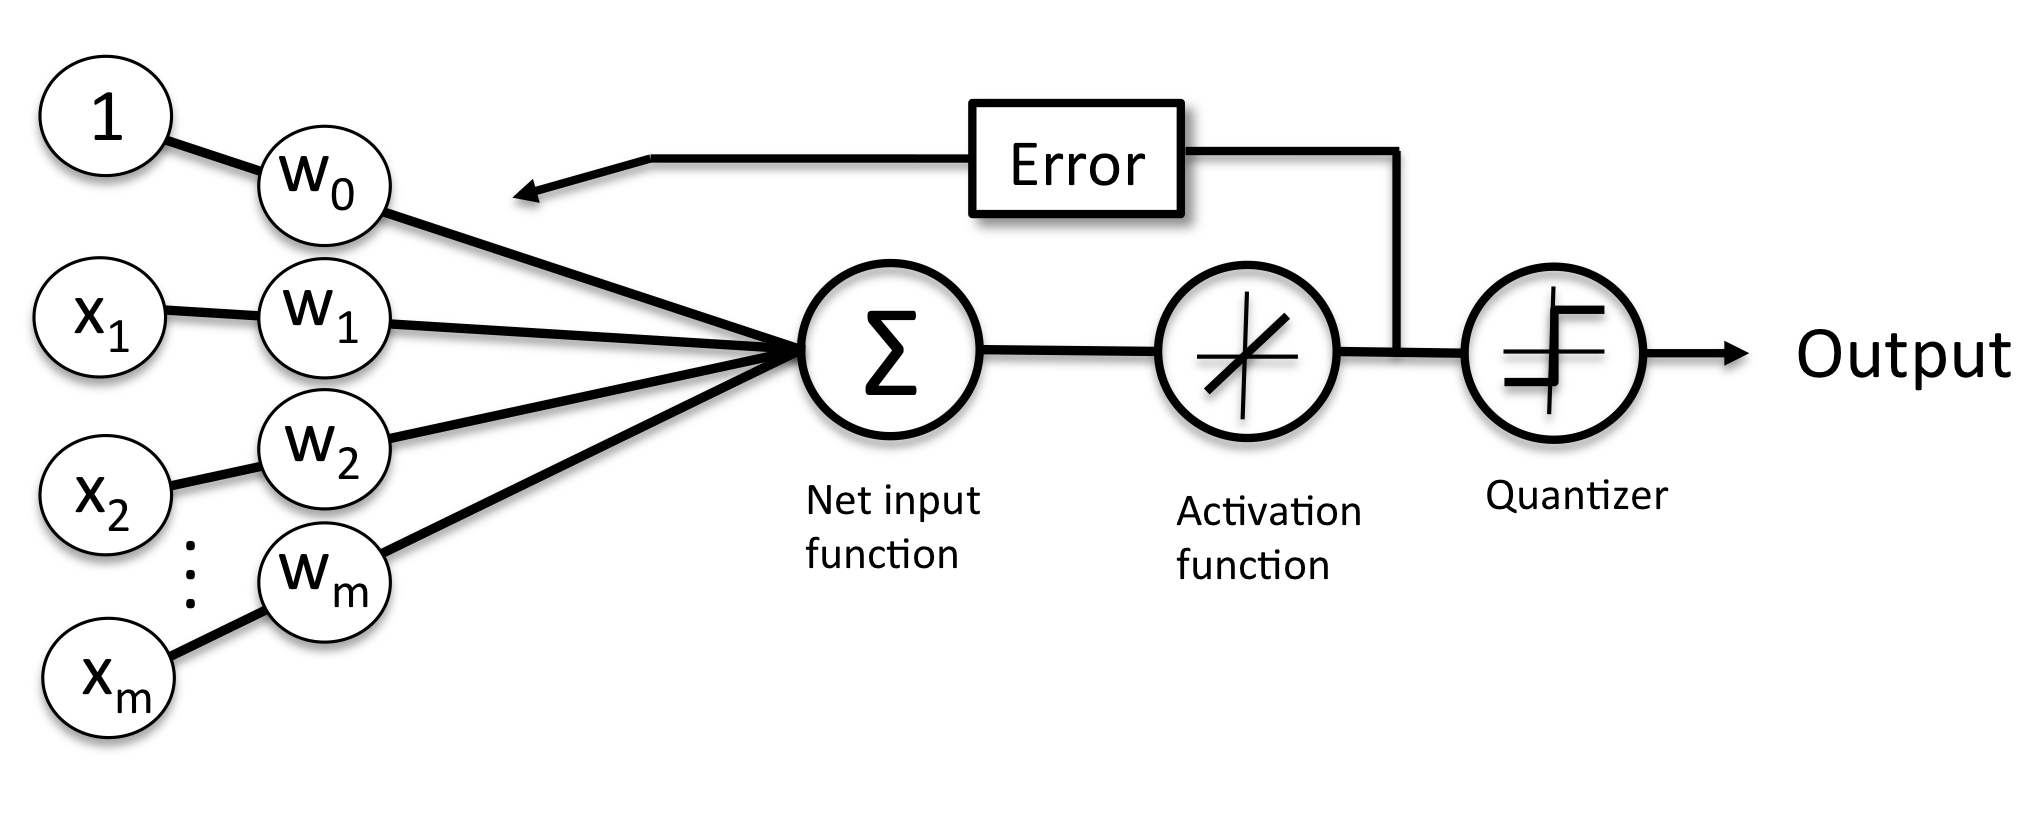
\includegraphics[width=.4\textwidth]{adaline-concept}
				\caption{General concept of adaline perceptron}
				\label{fig:adaline-concept}
			\end{figure}

			\paragraph{Cost function}

			\begin{figure}
				\centering
				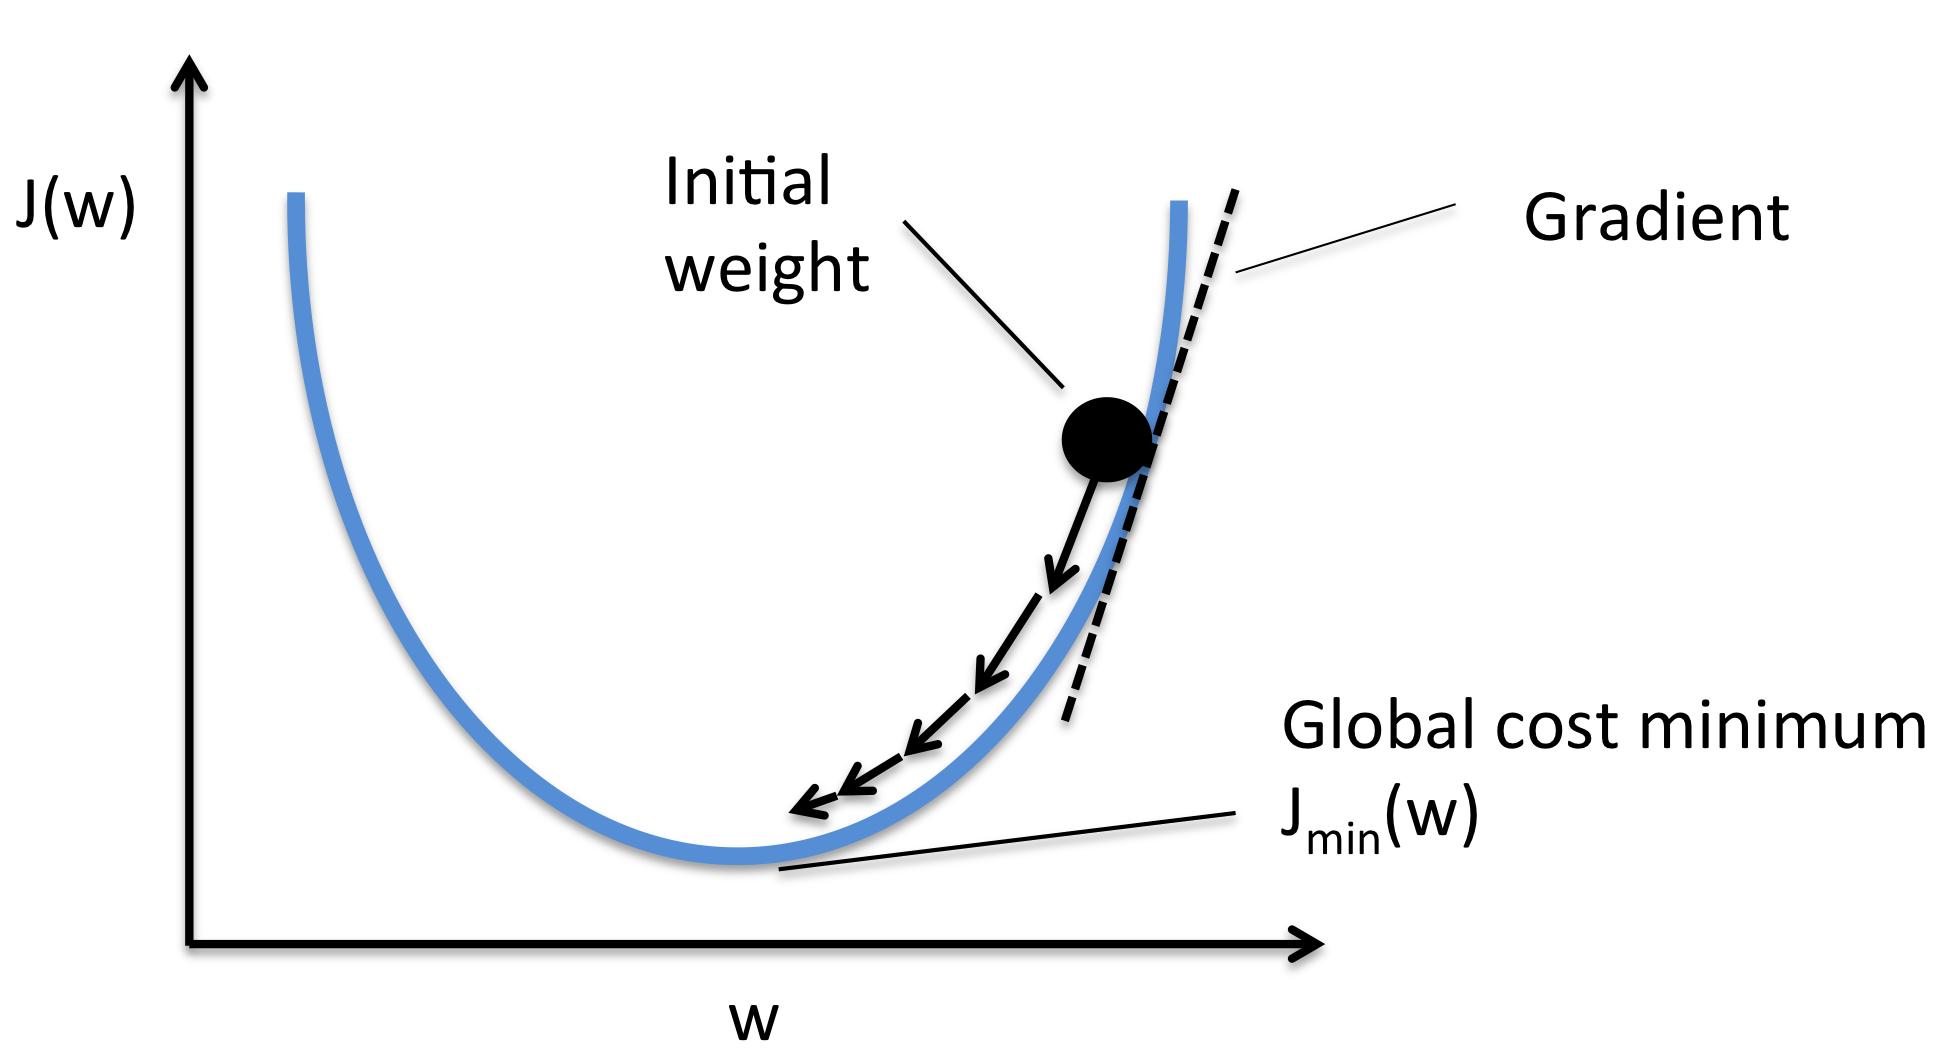
\includegraphics[width=.4\textwidth]{gradient-descend}
				\caption{Gradient descent}
				\label{fig:gradient-descend}
			\end{figure}

			\begin{equation}
				J(w) = \frac{1}{2} \sum_i (y^{(i)}-\phi(z^{(i)}))^2
			\end{equation}

			\paragraph{Update of weight vector}

			\begin{align}
					w_j &:= w_j + \Delta w_j \\
					\Delta w_j &= -\eta\nabla J(w) = \eta\sum_i (y^{(i)} -\phi(z^{(i)}))x^{(i)}_j
			\end{align}

			\paragraph{Features standarization}

			\begin{equation}
				x'_j = \frac{x_j - \mu_j}{\sigma_j}
			\end{equation}


			\subsubsection{Single Layer Neural Networks}
			\label{sec:single-layer-nn}


				\paragraph{Simple Perceptron}
				\label{sec:perceptron}
				[TODO ]

				\paragraph{ADALINE}
				\label{sec:adaline}
				[TODO ]

			\subsubsection{Multi Layer Perceptron}
			\label{sec:mlp}

				\paragraph{}
				[TODO ]

			\subsubsection{Radial Basis Functions}
			\label{sec:rbf}

				\paragraph{}
				[TODO ]

			\subsubsection{Convolutional Neural Networks}
			\label{sec:cnn}

				\paragraph{}
				[TODO ]

			\subsubsection{Recurrent Neural Networks}
			\label{sec:rnn}

				\paragraph{}
				[TODO ]

	\section{Unsupervised Learning}
	\label{sec:unsupervised-learning}

			\paragraph{}
			[TODO ]

%-----------------------------
%	Bibliographic references
%-----------------------------

	\nocite{subject:taa}
	\nocite{pactk:py-machine-learning}

  \bibliographystyle{alpha}
  \bibliography{bib}

\end{document}
